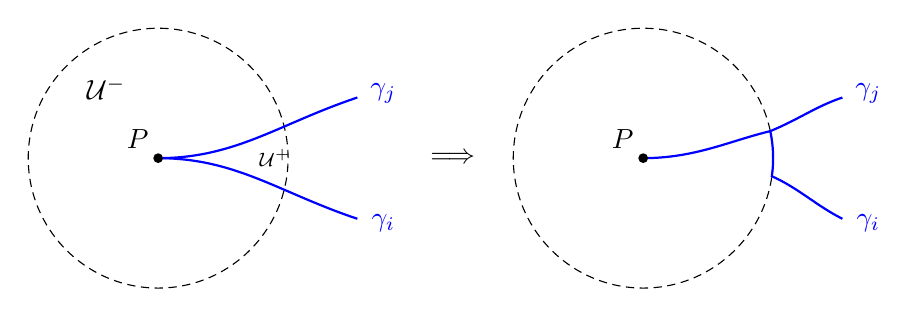
\begin{tikzpicture}[scale=1.1]
  % before: two arcs leave P tangentially (a cusp)
  \begin{scope}
    \draw[densely dashed] (0,0) circle (1.5);
    \draw[thick,blue] (0,0) .. controls (0.9,0) and (1.4,0.4) .. (2.3,0.7);
    \draw[thick,blue] (0,0) .. controls (0.9,0) and (1.4,-0.4) .. (2.3,-0.7);
    \node[blue] at (2.6,0.75) {$\gamma_j$};
    \node[blue] at (2.6,-0.75) {$\gamma_i$};
    \node[font=\scriptsize] at (1.35,0) {$\mathcal U^+$};
    \node at (-0.6,0.8) {$\mathcal U^-$};
    \fill (0,0) circle (1.6pt) node[above left] {$P$};
  \end{scope}
  \node at (3.4,0) {$\Longrightarrow$};
  % after: a single arc from P, branching near the boundary of the disc
  \begin{scope}[xshift=5.6cm]
    \draw[densely dashed] (0,0) circle (1.5);
    \draw[thick,blue] (0,0) .. controls (0.6,0) and (1.0,0.2) .. (12:1.5) .. controls (1.8,0.45) and (2.0,0.6) .. (2.3,0.7);
    \draw[thick,blue] (12:1.5) arc (12:-8:1.5) .. controls (1.8,-0.35) and (2.0,-0.55) .. (2.3,-0.7);
    \node[blue] at (2.6,0.75) {$\gamma_j$};
    \node[blue] at (2.6,-0.75) {$\gamma_i$};
    \fill (0,0) circle (1.6pt) node[above left] {$P$};
  \end{scope}
\end{tikzpicture}
